\documentclass[12pt,a4paper]{article}

% ─── Page Layout ───────────────────────────────────────────────────────────────
\usepackage[a4paper, margin=0.8in, headheight=14pt]{geometry}

% ─── Fonts (XeLaTeX) ───────────────────────────────────────────────────────────
\usepackage{fontspec}
\usepackage{unicode-math}
\setmainfont{TeX Gyre Pagella}
\setmonofont[Scale=0.88]{TeX Gyre Cursor}
\setmathfont{Latin Modern Math}

% ─── Packages ──────────────────────────────────────────────────────────────────
\usepackage{xcolor}
\usepackage{colortbl}
\usepackage{titlesec}
\usepackage{enumitem}
\usepackage{tabularx}
\usepackage{booktabs}
\usepackage{array}
\usepackage{amsmath}
\usepackage{tikz}
\usetikzlibrary{shapes.geometric, arrows.meta, positioning, calc, fit, decorations.pathreplacing, patterns}
\usepackage{tcolorbox}
\tcbuselibrary{skins, breakable}
\usepackage{hyperref}
\usepackage{fancyhdr}
\usepackage{graphicx}
\usepackage{microtype}
\hyphenpenalty=10000
\exhyphenpenalty=10000
\sloppy
\usepackage{caption}
\usepackage{setspace}
\usepackage{multirow}
\usepackage{tocloft}

% ─── Q&A helper ────────────────────────────────────────────────────────────────
\newcommand{\Q}[1]{\textbf{#1}\par\noindent\ignorespaces}

% ─── Colour Palette ────────────────────────────────────────────────────────────
\definecolor{myred}{RGB}{196,30,58}
\definecolor{mydark}{RGB}{30,30,50}
\definecolor{mygreen}{RGB}{14,120,80}
\definecolor{myteal}{RGB}{0,130,140}
\definecolor{myamber}{RGB}{180,100,0}
\definecolor{mypurple}{RGB}{100,30,160}
\definecolor{mygray}{RGB}{246,247,249}
\definecolor{mgframe}{RGB}{180,185,200}
\definecolor{watermark}{RGB}{145,150,170}
\definecolor{hdrred}{RGB}{250,232,235}
\definecolor{hdrgreen}{RGB}{220,244,233}
\definecolor{hdrteal}{RGB}{220,242,244}
\definecolor{hdramber}{RGB}{253,242,215}
\definecolor{hdrpurple}{RGB}{238,228,255}
\definecolor{hdrgray}{RGB}{238,240,245}
\definecolor{rowalt}{RGB}{250,251,253}

% ─── Section Formatting ────────────────────────────────────────────────────────
\titleformat{\section}
  {\large\bfseries\color{myred}}{\thesection.}{0.5em}{}
  [\vspace{1pt}{\color{myred}\rule{\linewidth}{0.8pt}}]
\titleformat{\subsection}
  {\normalsize\bfseries\color{myteal}}{\thesubsection}{0.5em}{}
\titlespacing*{\section}{0pt}{18pt}{7pt}
\titlespacing*{\subsection}{0pt}{11pt}{4pt}

% ─── Paragraph ─────────────────────────────────────────────────────────────────
\setlength{\parindent}{0pt}
\setlength{\parskip}{4pt}

% ─── TOC Styling ───────────────────────────────────────────────────────────────
\renewcommand{\cfttoctitlefont}{\large\bfseries\color{myred}}
\renewcommand{\cftaftertoctitle}{\par\noindent{\color{myred}\rule{\linewidth}{0.8pt}}}
\setlength{\cftbeforetoctitleskip}{0pt}
\setlength{\cftaftertoctitleskip}{6pt}
\renewcommand{\cftsecfont}{\normalsize\bfseries\color{mydark}}
\renewcommand{\cftsecpagefont}{\normalsize\bfseries\color{mydark}}
\renewcommand{\cftsecleader}{\cftdotfill{\cftdotsep}}
\setlength{\cftbeforesecskip}{7pt}
\renewcommand{\cftsubsecfont}{\small\color{mydark}}
\renewcommand{\cftsubsecpagefont}{\small\color{mydark}}
\setlength{\cftbeforesubsecskip}{3pt}
\setlength{\cftsubsecindent}{1.4em}

% ─── Table helpers ─────────────────────────────────────────────────────────────
\renewcommand{\arraystretch}{1.45}
\setlength{\tabcolsep}{6pt}
\arrayrulecolor{mydark}
\newcolumntype{B}[1]{>{\small\bfseries\raggedright\arraybackslash}m{#1}}
\newcolumntype{Y}{>{\small\raggedright\arraybackslash}X}
\renewcommand{\tabularxcolumn}[1]{m{#1}}

% ─── Header / Footer ───────────────────────────────────────────────────────────
\pagestyle{fancy}
\fancyhf{}
\fancyhead[L]{\small\color{myred}\textbf{26-ES-EE101}\;\color{mydark}--- Basic Electrical and Electronics Engineering}
\fancyhead[R]{\small\color{myteal}\textbf{Module 2 Notes}}
\fancyfoot[C]{\small\color{mydark}\thepage}
\fancyfoot[R]{\small\color{watermark}\textit{\copyright\ Biraj}}
\renewcommand{\headrulewidth}{0.5pt}
\renewcommand{\footrulewidth}{0.3pt}

% ─── Hyperref ──────────────────────────────────────────────────────────────────
\hypersetup{
  colorlinks=true, linkcolor=myteal, urlcolor=myteal,
  pdfauthor={Biraj Sarkar (CGEC)},
  pdftitle={26-ES-EE101 --- Module 2 Notes: Direct-Current Circuits}
}

% ─── tcolorbox styles ──────────────────────────────────────────────────────────
\tcbset{
  tikzbox/.style={
    colback=mygray, colframe=mgframe, boxrule=0.6pt, arc=4pt,
    left=8pt, right=8pt, top=6pt, bottom=6pt,
    colbacktitle=mgframe, coltitle=mydark, fonttitle=\small\bfseries
  },
  defbox/.style={
    colback=hdrgreen, colframe=mygreen, boxrule=0.8pt, arc=4pt,
    left=9pt, right=9pt, top=6pt, bottom=6pt,
    colbacktitle=mygreen, coltitle=white, fonttitle=\small\bfseries
  },
  formulabox/.style={
    colback=hdrteal, colframe=myteal, boxrule=0.8pt, arc=4pt,
    left=9pt, right=9pt, top=7pt, bottom=7pt,
    colbacktitle=myteal, coltitle=white, fonttitle=\small\bfseries
  },
  examplebox/.style={
    colback=hdramber, colframe=myamber, boxrule=0.8pt, arc=4pt,
    left=9pt, right=9pt, top=6pt, bottom=6pt,
    colbacktitle=myamber, coltitle=white, fonttitle=\small\bfseries
  },
  masonbox/.style={
    colback=hdrpurple, colframe=mypurple, boxrule=0.8pt, arc=4pt,
    left=9pt, right=9pt, top=6pt, bottom=6pt,
    colbacktitle=mypurple, coltitle=white, fonttitle=\small\bfseries
  },
  exambox/.style={
    colback=hdrpurple, colframe=mypurple, boxrule=1pt, arc=5pt,
    left=10pt, right=10pt, top=8pt, bottom=8pt,
    colbacktitle=mypurple, coltitle=white, fonttitle=\bfseries,
    breakable, title after break={\textbf{Frequently Asked / Viva Questions (contd.)}}
  }
}
\tcbset{breakable}
\tcbset{after={\par\color{black}}}

% ─── TikZ styles ───────────────────────────────────────────────────────────────
\tikzset{
  block/.style={rectangle, draw=myteal, fill=hdrteal,
    text width=2.4cm, align=center, minimum height=0.95cm,
    font=\small, rounded corners=3pt, line width=0.7pt},
  redblock/.style={rectangle, draw=myred, fill=hdrred,
    text width=2.4cm, align=center, minimum height=0.95cm,
    font=\small, rounded corners=3pt, line width=0.7pt},
  sumjunc/.style={circle, draw=myamber, fill=hdramber,
    minimum size=0.62cm, font=\small, line width=0.8pt},
  arrow/.style={-Stealth, thick, color=mydark},
  redarrow/.style={-Stealth, thick, color=myred},
  line/.style={thick, color=mydark}
}

\begin{document}

% ─── Title Page ───────────────────────────────────────────────────────────────
\begin{center}
  {\Large\bfseries\color{myred} 26-ES-EE101}\\[3pt]
  {\LARGE\bfseries\color{myred} Basic Electrical and Electronics Engineering}\\[5pt]
  {\normalsize\color{mydark} Semester I \quad$\bullet$\quad 3L:1T:0P \quad$\bullet$\quad 4 Credits}\\[3pt]
  {\normalsize\color{myteal}\textbf{Module 2 Exam Notes: Direct-Current Circuits}}\\[3pt]
  {\small\color{mydark} CGEC \;$|$\; MAKAUT Syllabus (A.Y. 2026--27) \;$|$\; \textit{Biraj Sarkar}}
\end{center}
\vspace{2pt}
\noindent{\color{myred}\rule{\linewidth}{1.5pt}}
\vspace{2pt}

\hypersetup{linkcolor=mydark}
\tableofcontents
\hypersetup{linkcolor=myteal}
\newpage

\section{Direct-Current Circuits}

\subsection{Circuit elements, signs and sources}
\begin{tcolorbox}[defbox,title={Passive sign convention}]
Mark the reference current entering the terminal labelled positive. Then \(p=vi\) is the power absorbed. A negative result means the element delivers power. References remain fixed even if calculated signs are negative.
\end{tcolorbox}

With voltage in volts, current in amperes and time in seconds, \(1\,\Omega=1\,\mathrm{V/A}\). Element laws under the passive sign convention are
\[
\begin{aligned}
v_R&=Ri_R, & p_R&=Ri_R^2,\\
v_L&=L\,\frac{di_L}{dt}, & W_L&=\frac12 Li_L^2,\\
i_C&=C\,\frac{dv_C}{dt}, & W_C&=\frac12 Cv_C^2 .
\end{aligned}
\]
Inductance \(L\) is measured in henries, capacitance \(C\) in farads, power in watts and energy in joules. In settled DC with finite values an ideal inductor has zero voltage and an ideal capacitor has zero current. Resistances add in series. Conductances \(G=1/R\), in siemens, add in parallel.

An independent source imposes its stated voltage or current. A dependent source sets its output by a circuit voltage \(v_x\) or current \(i_x\). The four types are
\[
\begin{aligned}
v_s&=\mu v_x &&\text{voltage-controlled voltage source},\\
i_s&=g_m v_x &&\text{voltage-controlled current source},\\
v_s&=r_m i_x &&\text{current-controlled voltage source},\\
i_s&=\beta i_x &&\text{current-controlled current source}.
\end{aligned}
\]
The gains \(\mu,\beta\) are dimensionless, \(g_m\) is in S and \(r_m\) in \(\Omega\). The standard symbol has a diamond outline with a polarity mark or an arrow. In circuit analysis keep dependent sources active. A source transformation exchanges a voltage source \(V_s\) in series with \(R\) for a current source \(I_s=V_s/R\) in parallel with \(R\), preserving the external terminal behaviour and polarity.

\subsection{Kirchhoff's laws and systematic analysis}
\begin{tcolorbox}[defbox,title={KCL and KVL}]
Kirchhoff's current law (KCL) says the algebraic sum of currents at a node is zero, by charge conservation. Kirchhoff's voltage law (KVL) says the algebraic sum of voltage changes around a closed loop is zero in the lumped circuit model.
\end{tcolorbox}

\textbf{Nodal analysis} is efficient when there are few essential nodes.
\begin{enumerate}[leftmargin=*, itemsep=3pt, topsep=4pt]
  \item Choose a reference node and label the unknown node voltages.
  \item Write KCL using currents such as \((V_a-V_b)/R\) from \(a\) to \(b\).
  \item If a voltage source joins two unknown nodes, use a \textbf{supernode}. Write KCL at its outer boundary and add the source equation \(V_a-V_b=V_s\) for the stated polarity.
\end{enumerate}

\textbf{Mesh analysis} applies to planar circuits.
\begin{enumerate}[leftmargin=*, itemsep=3pt, topsep=4pt]
  \item Assign clockwise mesh currents and write KVL for each mesh.
  \item In mesh 1, a resistor shared with mesh 2 gives the drop \(R(I_1-I_2)\).
  \item If a current source is shared, use a \textbf{supermesh}: write KVL around its outside and add \(I_1-I_2=I_s\) when the source points in the mesh-1 direction.
\end{enumerate}

\begin{tcolorbox}[tikzbox,title={Two-mesh circuit with a shared resistor},unbreakable]
\centering
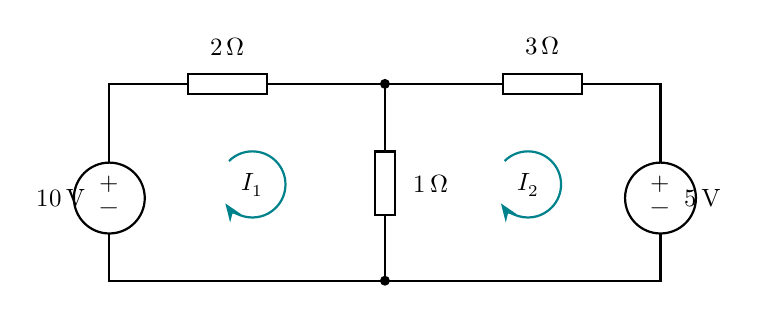
\begin{tikzpicture}[font=\small,line width=0.8pt]
\draw (0,1.5)--(0,2.5)--(1.0,2.5)
 (2.0,2.5)--(3.5,2.5)--(5.0,2.5)
 (6.0,2.5)--(7.0,2.5)--(7.0,1.5);
\draw (0,0.6)--(0,0)--(7.0,0)--(7.0,0.6);
\foreach \x/\volts/\side in {0/10/left,7/5/right}{
  \draw (\x,1.05) circle (0.45);
  \node at (\x,1.22) {$+$};
  \node at (\x,0.88) {$-$};
  \node[\side=5pt] at (\x,1.05) {$\volts\,\mathrm V$};
}
\draw (1.0,2.37) rectangle (2.0,2.63);
\draw (5.0,2.37) rectangle (6.0,2.63);
\node[above=3pt] at (1.5,2.63) {$2\,\Omega$};
\node[above=3pt] at (5.5,2.63) {$3\,\Omega$};
\draw (3.5,2.5)--(3.5,1.64) (3.5,0.83)--(3.5,0);
\draw (3.37,0.83) rectangle (3.63,1.64);
\node[right=3pt] at (3.63,1.23) {$1\,\Omega$};
\fill (3.5,2.5) circle (1.8pt) (3.5,0) circle (1.8pt);
\draw[-Stealth,myteal] (1.52,1.52) arc[start angle=135,end angle=-145,radius=0.42];
\node at (1.82,1.22) {$I_1$};
\draw[-Stealth,myteal] (5.02,1.52) arc[start angle=135,end angle=-145,radius=0.42];
\node at (5.32,1.22) {$I_2$};
\end{tikzpicture}
\end{tcolorbox}

\begin{tcolorbox}[examplebox,title={Find mesh currents and the shared-branch current}]
Take both top source terminals as positive and both mesh currents clockwise. Treat the source on the right as a \(5\,\mathrm V\) drop when traversed downwards.
\[
\begin{aligned}
2I_1+(I_1-I_2)&=10,\\
3I_2+(I_2-I_1)&=-5,\\
3I_1-I_2&=10,\qquad -I_1+4I_2=-5.
\end{aligned}
\]
\[
\begin{aligned}
I_2&=3I_1-10,\\
-I_1+4(3I_1-10)&=-5,\\
I_1&=\tfrac{35}{11}\,\mathrm A,\qquad I_2=-\tfrac{5}{11}\,\mathrm A,\\
I_{\mathrm{shared,down}}&=I_1-I_2=\tfrac{40}{11}\,\mathrm A.
\end{aligned}
\]
The right mesh current flows anticlockwise. Check by nodal analysis: the shared top node \(V\) satisfies
\[
\begin{aligned}
\tfrac{V-10}{2}+\tfrac{V-5}{3}+\tfrac{V}{1}&=0,\\
3(V-10)+2(V-5)+6V&=0,\\
V&=\tfrac{40}{11}\,\mathrm V.
\end{aligned}
\]
\end{tcolorbox}

\subsection{Star--delta transformation}
A star (Y) joins three arms \(R_a,R_b,R_c\) at an internal node. A delta (\(\Delta\)) joins the terminal pairs with resistances \(R_{ab},R_{bc},R_{ca}\). A transformation preserves resistance between any two terminals with the third terminal open. For example \(R_a+R_b=R_{ab}\parallel(R_{ca}+R_{bc})\). Write the two equivalent equations for the other pairs, add those involving terminal \(a\), subtract the remaining one, and divide by two to obtain the first formula below.

\begin{tcolorbox}[formulabox,title={Star--delta formulas}]
With \(S=R_{ab}+R_{bc}+R_{ca}\) and \(P=R_aR_b+R_bR_c+R_cR_a\),
\[
\begin{aligned}
R_a&=\frac{R_{ab}R_{ca}}{S},&
R_b&=\frac{R_{ab}R_{bc}}{S},&
R_c&=\frac{R_{bc}R_{ca}}{S},\\[3pt]
R_{ab}&=\frac{P}{R_c},&
R_{bc}&=\frac{P}{R_a},&
R_{ca}&=\frac{P}{R_b}.
\end{aligned}
\]
A balanced \(9\,\Omega\)-per-side delta becomes a \(3\,\Omega\)-per-arm star.
\end{tcolorbox}

\subsection{Superposition, Thevenin and Norton}
\begin{tcolorbox}[defbox,title={Three linear-network theorems}]
\textbf{Superposition.} A branch voltage or current in a linear circuit is the signed sum of the responses to each independent source acting alone.

\textbf{Thevenin.} A linear two-terminal circuit can be represented by an ideal voltage \(V_{\mathrm{th}}\) in series with \(R_{\mathrm{th}}\), when a finite Thevenin resistance exists.

\textbf{Norton.} The corresponding current-source model is \(I_{\mathrm N}\) in parallel with \(R_{\mathrm N}=R_{\mathrm{th}}\), when the Norton model is finite.
\end{tcolorbox}

\begin{itemize}[leftmargin=*, itemsep=3pt, topsep=4pt]
  \item \textbf{Superposition.} Short ideal independent voltage sources and open ideal independent current sources that are turned off. Keep dependent sources active. Sum signed voltage or current contributions before calculating power.
  \item \textbf{Thevenin voltage.} Disconnect the load and find the open-circuit voltage \(V_{\mathrm{oc}}\).
  \item \textbf{Port resistance.} Deactivate independent sources. With dependent sources present, drive the port with a test source and use \(R_{\mathrm{th}}=V_t/I_t\), with test current entering the port.
  \item \textbf{Norton current and cross-check.} \(I_{\mathrm N}=I_{\mathrm{sc}}\) supplied to an external short. If \(I_{\mathrm{sc}}\ne0\), \(R_{\mathrm{th}}=V_{\mathrm{oc}}/I_{\mathrm{sc}}\).
\end{itemize}

\begin{tcolorbox}[examplebox,title={From voltage divider to load power}]
A \(12\,\mathrm V\) source feeds a \(4\,\Omega\) series resistor and a \(6\,\Omega\) shunt resistor. The load is across the shunt.
\[
\begin{aligned}
V_{\mathrm{th}} &=12\frac{6}{4+6}=7.2\,\mathrm V,\\
R_{\mathrm{th}} &=4\parallel 6=\frac{4(6)}{4+6}=2.4\,\Omega,\\
I_{\mathrm N} &=\frac{7.2}{2.4}=3\,\mathrm A.
\end{aligned}
\]
For \(R_L=3.6\,\Omega\), \(I_L=7.2/(2.4+3.6)=1.2\,\mathrm A\).
The load power is \(I_L^2R_L=5.184\,\mathrm W\).
\end{tcolorbox}

\begin{tcolorbox}[examplebox,title={Superposition with voltage and current sources}]
A \(12\,\mathrm V\) source feeds a node through \(3\,\Omega\). A \(6\,\Omega\) resistor connects the node to ground. A \(1\,\mathrm A\) source injects current into the node from ground.
\[
\begin{aligned}
V^{(12\mathrm V)} &= 12\frac{6}{3+6}=8\,\mathrm V
     &&\text{(open the current source)},\\
V^{(1\mathrm A)} &=1(3\parallel6)=2\,\mathrm V
     &&\text{(short the voltage source)},\\
V&=8+2=10\,\mathrm V.
\end{aligned}
\]
Check KCL: \((10-12)/3+10/6-1=0\,\mathrm A\). Power in the \(6\,\Omega\) branch is \(10^2/6=16.67\,\mathrm W\) using the total voltage.
\end{tcolorbox}

\subsection{Maximum power transfer}
For a positive \(R_{\mathrm{th}}\) and a variable resistive load, the load receives maximum power at \(R_L=R_{\mathrm{th}}\):
\[
\begin{aligned}
P_L&=\frac{V_{\mathrm{th}}^2R_L}{(R_{\mathrm{th}}+R_L)^2},\\
\frac{dP_L}{dR_L}
 &= V_{\mathrm{th}}^2
   \frac{R_{\mathrm{th}}-R_L}{(R_{\mathrm{th}}+R_L)^3},\\
R_{L,\mathrm{opt}}&=R_{\mathrm{th}},&
P_{\max}&=\frac{V_{\mathrm{th}}^2}{4R_{\mathrm{th}}}.
\end{aligned}
\]
For nonzero source voltage the derivative changes from positive to negative. In the equivalent series circuit half the power is dissipated internally at this point. In the voltage-divider example the optimum is \(2.4\,\Omega\) and \(P_{\max}=5.4\,\mathrm W\).

\subsection{First-order RL and RC transients}
A \textbf{transient} is the temporary response after switching. Capacitor voltage and inductor current remain continuous for finite currents and voltages.
\begin{enumerate}[leftmargin=*, itemsep=3pt, topsep=4pt]
  \item Choose the state \(x=v_C\) or \(x=i_L\) and find \(x(0^+)=x(0^-)\) from the pre-switch circuit.
  \item Find \(x_\infty\) from the new DC circuit.
  \item Use the resistance \(R_{\mathrm{eq}}\) seen by the storage element after switching. Calculate \(\tau=R_{\mathrm{eq}}C\) for RC or \(\tau=L/R_{\mathrm{eq}}\) for RL, in seconds.
\end{enumerate}
\[
\begin{aligned}
\frac{dx}{dt}+\frac{x}{\tau}&=\frac{x_\infty}{\tau},\\
\frac{d}{dt}(x-x_\infty)&=-\frac{x-x_\infty}{\tau},\\
x(t)&=x_\infty+[x(0^+)-x_\infty]e^{-t/\tau}.
\end{aligned}
\]
The remaining difference from steady state at \(t=\tau\) is \(e^{-1}\) times the initial difference. After \(5\tau\) it is about \(0.67\%\).

\begin{tcolorbox}[tikzbox,title={Normalised first-order step responses},unbreakable]
\centering
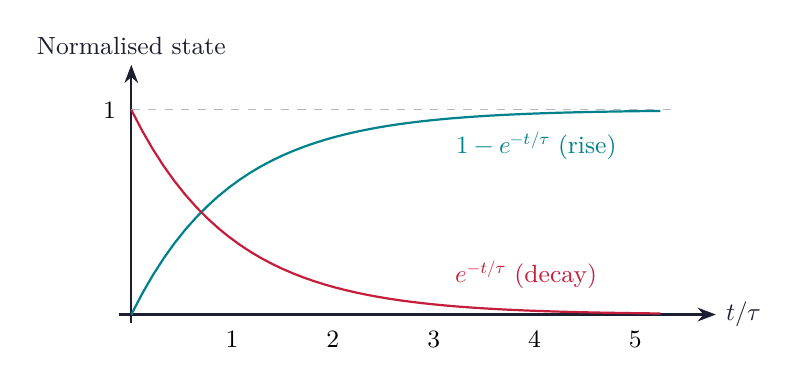
\begin{tikzpicture}[x=1.28cm,y=2.6cm,font=\small]
\draw[arrow] (-0.12,0)--(5.8,0) node[right] {$t/\tau$};
\draw[arrow] (0,-0.04)--(0,1.22) node[above] {Normalised state};
\draw[mgframe,dashed] (0,1)--(5.35,1);
\foreach \t in {1,2,3,4,5} \node[below] at (\t,-0.03) {\t};
\node[left=2pt] at (0,1) {1};
\draw[myteal,thick,domain=0:5.25,samples=50] plot (\x,{1-exp(-\x)});
\draw[myred,thick,domain=0:5.25,samples=50] plot (\x,{exp(-\x)});
\node[myteal,below] at (4.02,0.94) {$1-e^{-t/\tau}$ (rise)};
\node[myred,above] at (3.92,0.08) {$e^{-t/\tau}$ (decay)};
\end{tikzpicture}
\end{tcolorbox}

\begin{tcolorbox}[examplebox,title={Time constants and initial conditions},unbreakable]
An initially uncharged \(100\,\mu\mathrm F\) capacitor charges from \(10\,\mathrm V\) through \(2\,\mathrm{k}\Omega\).
\[
\begin{aligned}
\tau&=(2000)(100\times 10^{-6})=0.20\,\mathrm s,\\
v_C(t)&=10(1-e^{-t/0.20})\,\mathrm V,\\
v_C(0.20\,\mathrm s)&=6.32\,\mathrm V.
\end{aligned}
\]
For an RL step of \(12\,\mathrm V\), \(R=6\,\Omega\), \(L=3\,\mathrm H\), and \(i_L(0)=0\), the final current is \(2\,\mathrm A\) and \(\tau=0.50\,\mathrm s\). Thus \(i_L(t)=2(1-e^{-t/0.50})\,\mathrm A\).
\end{tcolorbox}

\newpage
\begin{center}
  {\large\bfseries\color{myred} Quick Revision --- Module 2}\\[3pt]
  {\small\color{mydark} Direct-Current Circuits $|$ 26-ES-EE101}
\end{center}
\noindent{\color{myred}\rule{\linewidth}{1.2pt}}
\vspace{4pt}

\begin{tcolorbox}[formulabox, title={Key Formulas and Concepts at a Glance}]
\renewcommand{\arraystretch}{1.35}
\begin{tabularx}{\linewidth}{B{4.4cm}Y}
Node current & $i_{ab}=(V_a-V_b)/R$ in A. \\[3pt]
Two-terminal equivalent & $V_{\mathrm{th}}=V_{\mathrm{oc}}$, $I_{\mathrm N}=I_{\mathrm{sc}}$. \\[3pt]
Maximum DC load power & $R_L=R_{\mathrm{th}}$, $P_{\max}=V_{\mathrm{th}}^2/(4R_{\mathrm{th}})$. \\[3pt]
Time constants & $\tau_{\mathrm{RC}}=RC$, $\tau_{\mathrm{RL}}=L/R$ in s. \\[3pt]
\end{tabularx}
\end{tcolorbox}

\begin{tcolorbox}[defbox, title={One-Line Definitions}]
\textbf{Mesh.} A loop in a planar circuit that encloses no smaller loop.

\textbf{Reference node.} The node assigned zero potential for the calculation.

\textbf{Time constant.} Time for the remaining first-order transient to fall to one over e of its initial value.
\end{tcolorbox}

\begin{tcolorbox}[exambox, title={Frequently Asked / Viva Questions}]
\begin{enumerate}[topsep=0pt, label=\textbf{Q\arabic*.}, itemsep=5pt]
  \item \Q{What physical principle gives KCL?} Conservation of charge at a node.
  \item \Q{What physical principle gives KVL?} A closed path has zero net voltage change in the lumped circuit model.
  \item \Q{When is a supernode used?} When an ideal voltage source joins two non-reference nodes.
  \item \Q{What makes a supermesh?} A current source lies on the boundary shared by two meshes.
  \item \Q{Can a dependent source be deactivated in superposition?} Keep its controlling relation active for each source contribution.
  \item \Q{Why superpose current before power?} Power is nonlinear in the branch current, for example $P=I^2R$.
  \item \Q{How do we find port resistance with a dependent source?} Turn off independent sources and apply a test source at the port.
  \item \Q{When is maximum power transferred to a resistive load?} When the positive load resistance equals the positive Thevenin resistance.
  \item \Q{Which two quantities are continuous at normal switching?} Inductor current and capacitor voltage.
  \item \Q{What are the settled DC models for L and C?} An ideal inductor is a short circuit and an ideal capacitor is an open circuit.
\end{enumerate}
\end{tcolorbox}

\begin{tcolorbox}[tikzbox, title={Summary Reference}]
\begin{tabularx}{\linewidth}{|B{4.0cm}|Y|}\hline
Topic & \textbf{What to remember} \\ \hline
Nodal method & Write KCL in terms of voltages and add source constraints. \\ \hline
Mesh method & Write KVL in terms of mesh currents and add current-source constraints. \\ \hline
Network equivalent & Remove the load, calculate port values, then reconnect the load. \\ \hline
\end{tabularx}
\end{tcolorbox}

\end{document}

